\section{Background}

Our work focuses on energy saving in cloud storage systems through the use of
block level caching mechanisms. We use DM-Cache as the block level caching
mechanism to evaluate our work on as it is freely available as a Linux kernel
module and is currently in use in many cloud storage systems such as Facebook's
FlashCache which is based on the implementation of DM-Cache \cite{flashcache}.

\subsection{Storage Area Networks}

Due to the physical limitation of local storage, many enterprise solutions
choose to emply Storage Area Networks, or SAN's, in an attempt to centralize
storage access and provide larger storage capabilities. SAN's also provide for
simplification of virtual machine migration and increased data reliability. Due
to the central nature of the storage this means that multiple nodes will use the
same storage node for all their data needs. For the storage node this means
satisfying multiple requests from many different machines and being able to do
so quickly. Because the storage is no longer local this increases request
latency as the storage node is further from the client and has to service
multiple clients at a time. With this kind of storage bottlenecks such as
network bandwidth and I/O throughput can play large roles in both performance
and power consumtion.

\subsection{Local SSD Caching}

Usage of SSD's as primary storage is impractical because of cost and storage
size. The cost of an SSD per gigabyte is much higher than that of conventional
HDD's and their storage size is very limited compared to multi terrabyte hard
disks. SSD performance is much higher than HDD's as there are no mechanical
parts which makes them ideal to use as cache devices.

Using an SSD as a local cache device diverts some read requests from the
mechanical drive to the much faster and more energy efficient SSD. The more
requests that can be satisfied using the local cache device the higher the
performance gains for the workload. This also saves energy as the requests are
now being satisfied by a more power efficient storage mechanism than standard
mechanical drives.

\subsection{DM-Cache}

\begin{figure}
  \caption{Architecture of DM-Cache}
  \centering 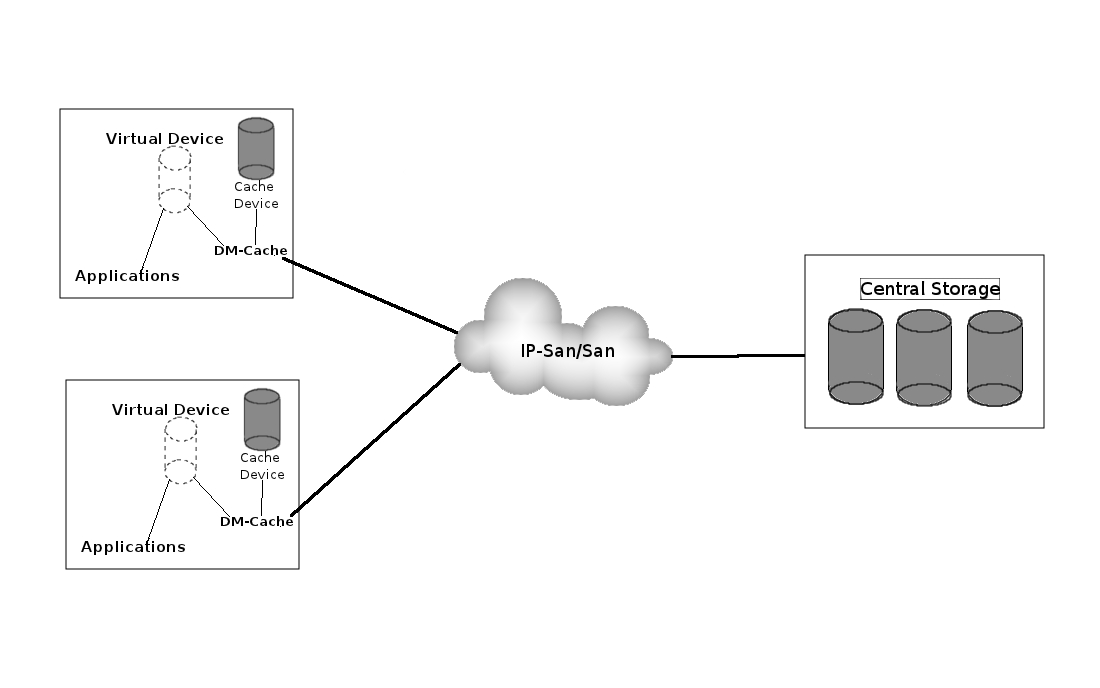
\includegraphics[width=0.5\textwidth]{dm-cache_diagram.jpg}
  \label{fig:dm-cache}
\end{figure}

DM-Cache, or Device Mapper Cache, is a block-level caching mechanism implemented
as a module in the Linux kernel \cite{DM-Cache}. It allows for specification of
a local SSD as a cache device where recently used blocks can be stored for
faster access time. It supports both write-back and write-through functionality
for handling cached data. Figure~\ref{fig:dm-cache} shows the architecture of
DM-Cache.

The purpose of DM-Cache is to cache recently used blocks on local storage
instead of retrieving them from some external storage source. This helps to
alleviate network bandwidth issues as well as reduce response times and save
power by issuing less requests to the storage nodes which use mechanical disks.

The current implementation of DM-Cache uses a hash table that maps logical block
addresses to entries within the hash table and evictions are done when two block
addresses map to the same entry but contain different data. This eviction scheme
does not take into account most recently used blocks and it also does not make
any attempt to pre-fetch any other blocks. Our work expands DM-Cache's cache
eviction policy to make smarter decisions in order to increase performance and
save energy.
